\documentclass{article}
\usepackage{nips_2016}
\usepackage[utf8]{inputenc} % allow utf-8 input
\usepackage[T1]{fontenc}    % use 8-bit T1 fonts
\usepackage{hyperref}       % hyperlinks
\usepackage{url}            % simple URL typesetting
\usepackage{booktabs}       % professional-quality tables
\usepackage{amsfonts}       % blackboard math symbols
\usepackage{nicefrac}       % compact symbols for 1/2, etc.
\usepackage{microtype}      % microtypography
\usepackage{graphicx}
\usepackage{float}
\usepackage{subcaption}
\setlength{\belowcaptionskip}{-10pt}

\title{ML Project - Embedding music for automatic composition spaces}
\author{Thomas Guennoc \and Laure Pretet \and Pierre Rampon } 
\date{\today}

\begin{document}
\maketitle

\newpage

\tableofcontents

\newpage

\section{Introduction}

\hspace{0.5cm}Our objective with this project is to provide digital tools for music understanding and composition. These tools could help humans but also computers, as it could improve the quality of automatic music generation. 

\hspace{0.5cm}More precisely, our programs will have to find patterns in the way notes and chords follow one an other. We will use machine learning related knowledge, and more specifically Convolutional Neural Networks (CNN), to reach this goal. Once we have more information about the musical patterns in a musical genre, it's easier to obtain a succession of musical elements that makes sense, using random walks.

\hspace{0.5cm}In this document we will discuss about both music and informatics. More precisely, we will deal with symbolic music and use the MIDI encoding to do so. For the sake of simplicity and to remain very symbolic, we ignored timbre, velocity and octaves changes.

\section{Creating a toy dataset}
\subsection{Which data ?}

\hspace{0.5cm}Machine learning algorithms can perform many tasks, by using and organizing information contained in already existing data. The bigger the set of labeled samples they get, the more they can improve. Here, as a first approach to the problem, we want to generate a wide yet simple set of harmonic progressions, using specific musical scales. First, the generated dataset is pretty simple and can't be used to train neural networks properly, but they are a first step toward mastering the digital tools needed (midi encoding, neural network libraries) to implement more complex algorithms.

\hspace{0.5cm} To start having an understanding of music, we chose to use the chords as basic elements and study how to combine them. To train our embedding space understand this logic, we chose to train it to predict the next chord in a sequence of chords. So we built a prediction dataset.

\hspace{0.5cm}The code we implemented allows us to generate MIDI harmonic progressions. These are sequences of chords which musically make sense, and which were extracted from our personal musical knowledge. They have a fixed number of beats and a basic rhythm : one chord per beat. The training chords are built from a musical scale and a list of integers, representing the degree of the fundamental note of each chord. For instance, the sequence of chords Em, D, C and Am shown in figure \ref{eiffel} is built from a minor scale and the list $[0,6,5,3]$. The dimension of the dataset was enhanced by :
\begin{itemize}
\item circular permutations
\item transpositions
\end{itemize}

This approach to building dataset was inspired from the \textit{dSprites} images dataset.

\begin{figure}[H]
\centering
\includegraphics[width =0.5\textwidth]{eiffelmelo.png}
\caption{Chords from Eiffel65 - I'm Blue, seen on FL Studio piano roll}
\label{eiffel}
\end{figure}

\subsection{Which musical genre ?}
\hspace{0.5cm}Each specific musical genre having its own specific patterns, it seems unrealistic to create an algorithm able to work for every kind of music. We can imagine that more developped algorithms need to focus on a genre, as different chords may be expected at some moments, depending on the kind of music. Some of us suggested we base our work on jazz tracks, as it involves many different chords and rhythmic structures. Pop music may also be interesting : as it uses mainly major and minor chords in a regular way, it could be simpler to study at first. That's why our toy dataset contains many pop progressions. Either way, the algorithm can easily be accommodated to an other musical genre by changing the basis of harmonic progressions. 

\hspace{0.5cm} However, some musical genres require to have a very specific rhythm (consider the bossa nova, the "groove" in jazz), and in this case, we would need to implement multiple durations as well.

\subsection{How to train ?}
\hspace{0.5cm}We organised our data in such a way that the network can be trained by prediction. If our progressions have a fixed length N, the training data will be the first N-1 chords, while the expected label will be the last chord, which normally follows the others. The melodies in our dataset can have different lengths but we loop on them the right number of times, so that the resulting progressions are all the same size (N).

\begin{figure}[H]
\centering
\includegraphics[width =1\textwidth]{ex_n_eg_10.png}
\caption{Chords extracted from Eiffel65 - I'm Blue. We loop two times and a half over the melody of 4 chords to reach $N=10$}
\label{eiffelprog}
\end{figure}

\subsection{Which results to expect ?}\label{expectations}

\hspace{0.5cm}For the validation of the model, we were guided by the work of the project GloVe \cite{pennington2014glove} on natural language semantics. The networks trained by them was able to organize words according to the meaning they convey, and thus to identify patterns called \textit{linear substructures}. For example, the superlative of a word, the link between a country and its capital city ...

\hspace{0.5cm} In a similar way, we tried to identify such relationships that can exist between two chords in music. Now we can expect our network to be able to establish relationships between :

\begin{itemize}
\item A chord and the pitch it contains
\item Major/Minor
\item First degree/Fifth degree (authentic cadence)
\item Third and Fifth chord of a same tonality
\item L, P or R (links in the Tonnetz)
\item Morphological operations (like inversions in the circle, cf. Moreno Andreatta's lecture)
\item Chords having notes in common
\end{itemize}

These properties must remain independent from the pitch (the transposition). They must be useful to predict a note or a chord. Let's take an exemple of a useful property : if we consider again the score of Eiffel65 - I'm Blue, we can see on the figure \ref{eiffelfull} that the notes of the melody are basically the notes of the 3-notes-chord playing at the same time. Hence, if we were to predict the notes, it would be convenient to use an established relationships between a chord and its individual notes. We can easily expect a B if an E chord is being played at the time, as we can easily expect "Paris" if the words "France" and "capital" have been said before. Speaking of useful musical properties, we can also see on figure \ref{eiffelfull} that the chords shares many notes with each other (the C and Am chords both contains a C and a E for example).

\begin{figure}[H]
\centering
\includegraphics[width =0.8\textwidth]{eiffelfullmelo.png}
\caption{Horizontal zoom on the chords (green) and the melody (red) of Eiffel65 - I'm Blue.}
\label{eiffelfull}
\end{figure}

\section{Getting familiar with the models}

\subsection{Recurrent networks}

At first, we tried to execute generic tasks with RNNs and LSTMs : text prediction and midi chords prediction. We implemented our own RNN and LSTM cells and compared performances of all four networks.

\begin{figure}[H]
\centering
\includegraphics[width =1\textwidth]{Ex2Sherlock.eps}
\caption{Performances of simple prediction networks on a text dataset}
\label{rnnstext}
\end{figure}

On this first figure, we can clearly see how the network is able to adapt to the training data. It is also able to generalize to unknown validation data. But after a certain number of iterations (typically 10 epochs), the loss curve on validation crosses the one of training data. After this point, training loss will continue to decrease, but validation loss will stagnate. The network will overfit. \\
These models reach between 20\% and 26\% accuracy. \\

\textbf{NB.} On \ref{rnnstext}, and \ref{rnnmidi0}, the validation loss is lower than the training loss at the beginning. This is because the loss is computed using a simple cumulated Mean Square Error and the validation dataset is smaller than the training dataset. So we will focus on the trends expressed by both curves.

\begin{figure}[H]
\centering
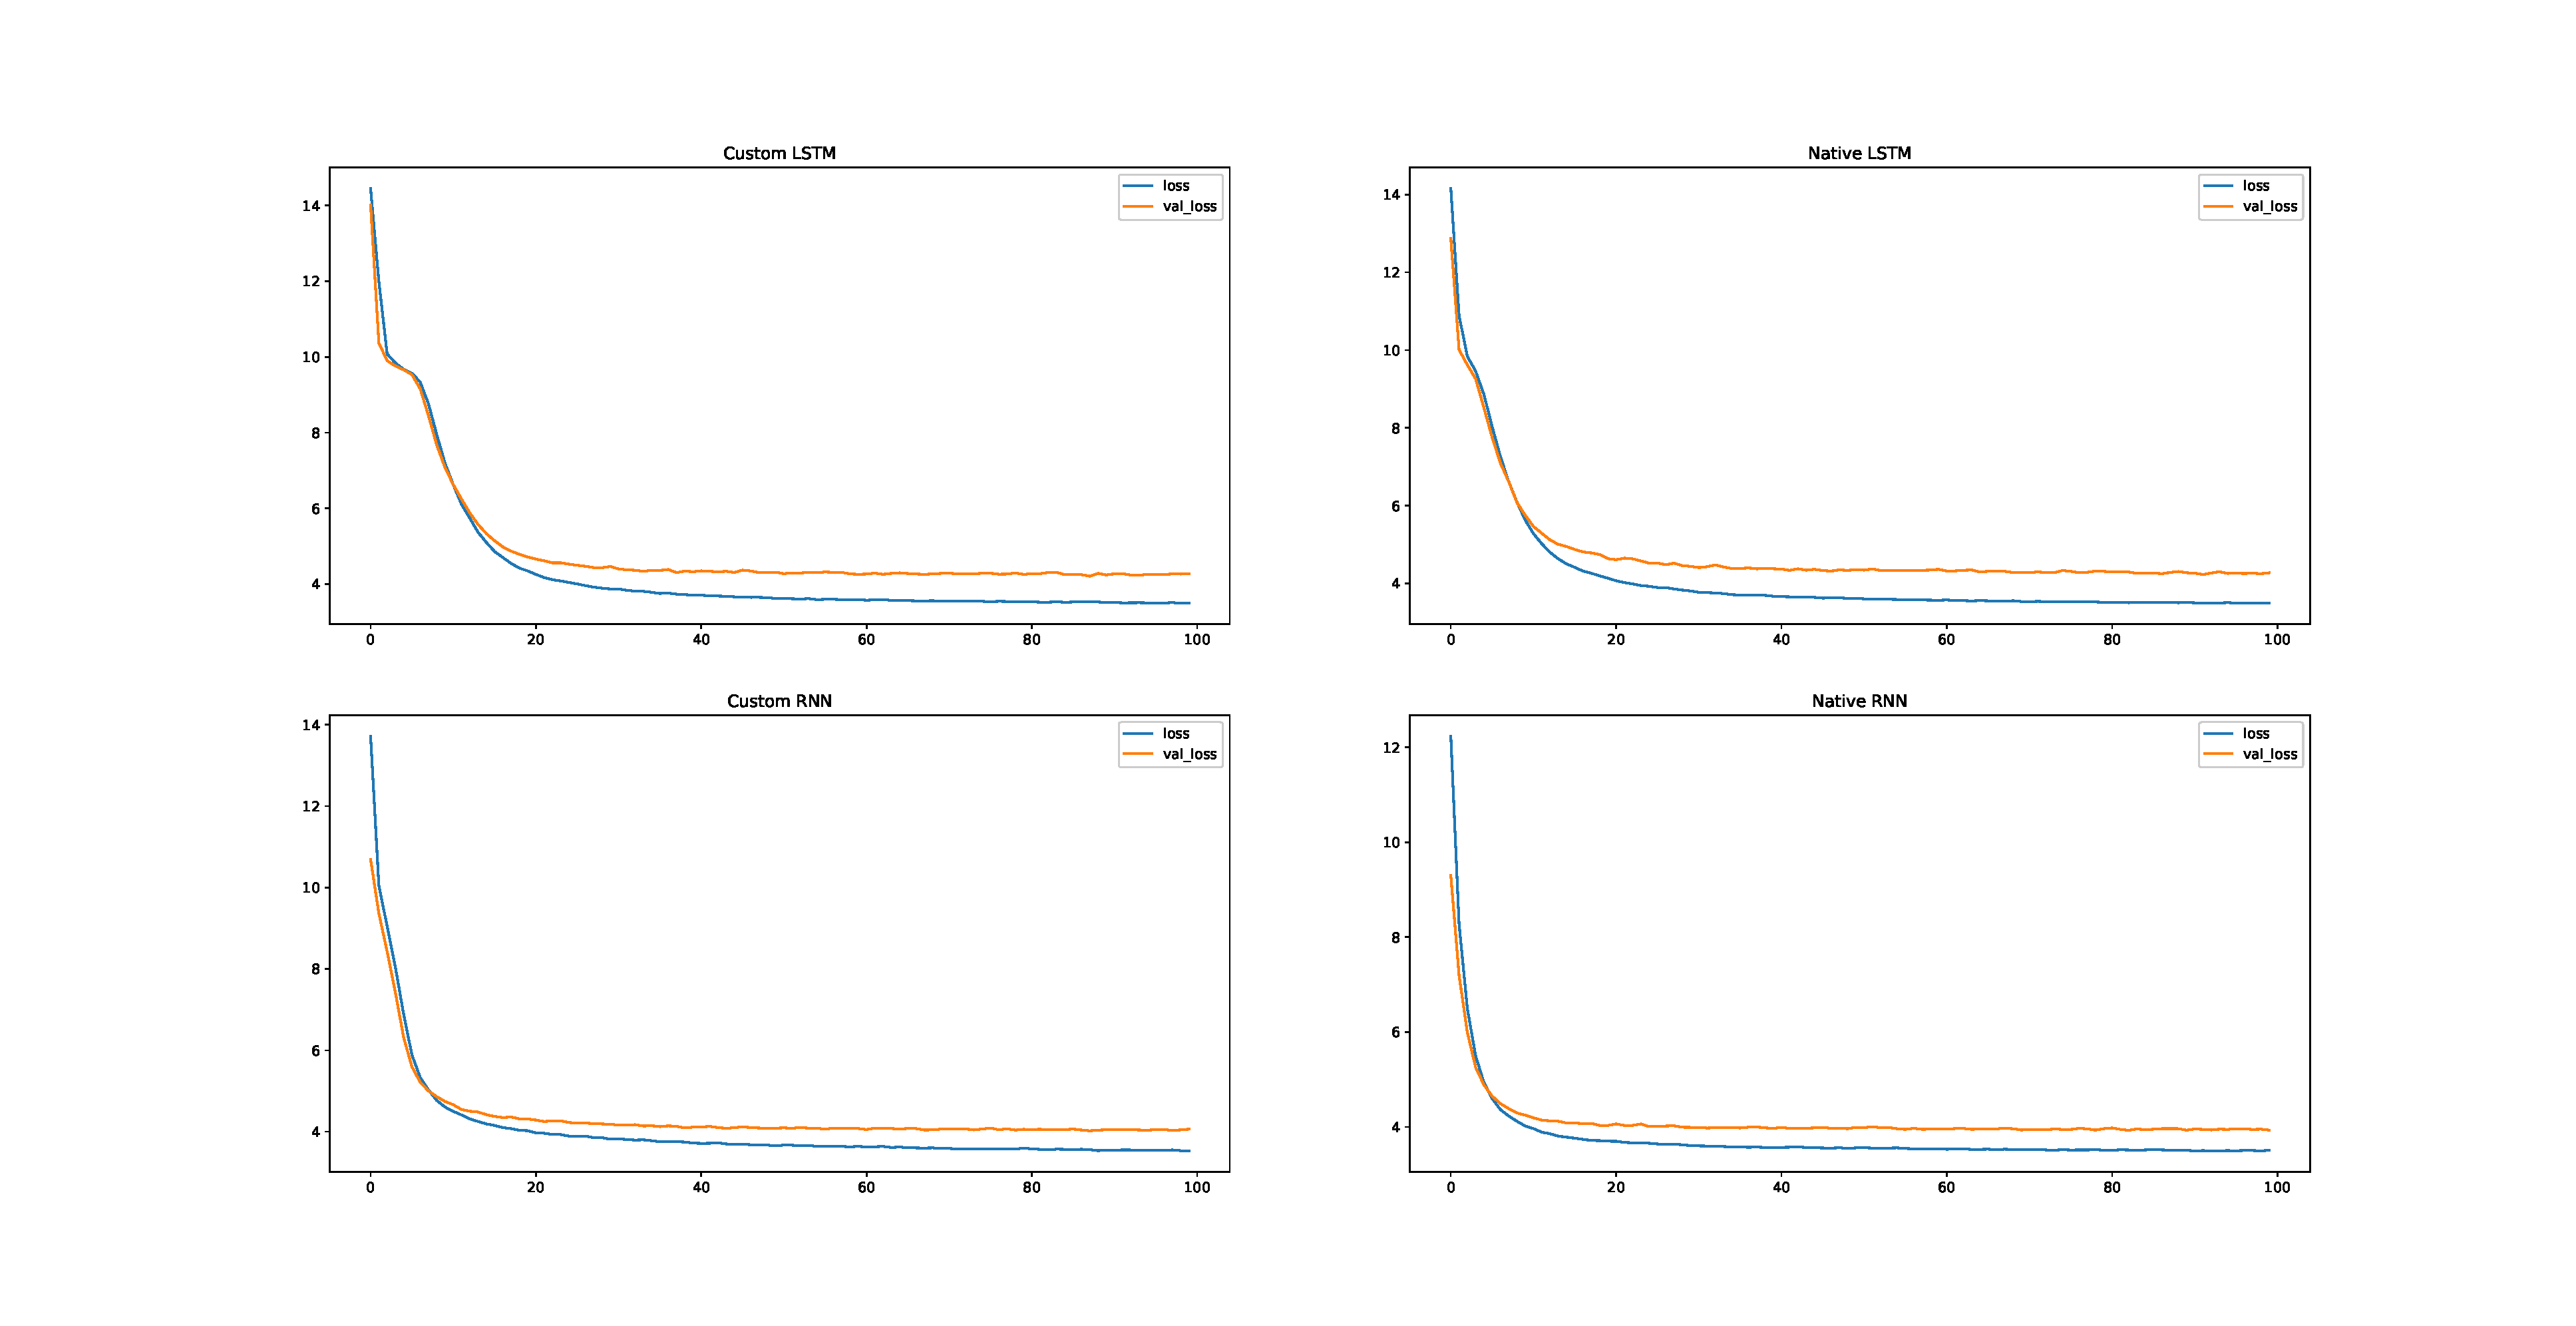
\includegraphics[width =1\textwidth]{Ex2Midi.eps}
\caption{Performances of simple prediction networks on our midi chord progressions dataset}
\label{rnnmidi0}
\end{figure}

By using the MIDI toy dataset, we were able to run more iterations and confirm that the overfitting point for this configuration is located between 10 and 20 iterations. \\
These models reach about 30\% accuracy.

\subsection{Convolutional networks}

To implement our first CNN, we inspired ourselves by a tutorial (\href{https://medium.com/@thoszymkowiak/how-to-implement-sentiment-analysis-using-word-embedding-and-convolutional-neural-networks-on-keras-163197aef623}{imdb cnn}). It was supposed to perform sentiment analysis on IMDB movie review. This network works fine, except it seems to have some little underfitting issue. Still, it is able to provide more than 85\% accuracy on the validation data. However, when we tried to use the exact same network on our data, the results were catastrophic (no more than 7 \% accuracy). We deduced that this model was not suited to our problem.

\begin{figure}[H]
\centering
\begin{subfigure}{.5\textwidth}
  \centering
  \includegraphics[width =1\linewidth]{ImdbCNN.eps}
  \caption{Sentiment classification task}
  \label{fig:sub1}
\end{subfigure}%
\begin{subfigure}{.5\textwidth}
  \centering
  \includegraphics[width=1\linewidth]{MidiCNN0.eps}
  \caption{Midi chords prediction task}
  \label{fig:sub2}
\end{subfigure}
\caption{Performances of a simple convolutional network}
\label{fig:cnns}
\end{figure}

So we changed the model to make fit out data. In particular :

\begin{itemize}
\item We used MSE loss (categorical cross-entropy is not designed to make prediction).
\item We used Adagrad or RMSPROP optimizer (they perform better than Adam for very sparse data like ours).
\item We changed the filter size : 3 was suited to images and text, but for Midi notes, we need to span at least on 12 (an octave) in order to catch the meaning of a chord.
\item We added a pooling layer.
\item We used a "sequencer" for prediction (TimeDistributed layer wrapper in Keras). It means that the convolution and pooling operations preserve the time dimension of the data. (We removed the pooling layer at this step because both features were hardly compatible).
\end{itemize}

Eventually we obtained satisfying results :

\begin{figure}[H]
\centering
\includegraphics[width =1\textwidth]{MidiCNN.eps}
\caption{Performances of the new networks on our midi chord progressions dataset}
\label{rnnmidi}
\end{figure}

By this time, the architecture evolved from \ref{fig:sub3} to \ref{fig:sub4} :

\begin{figure}[H]
\centering
\begin{subfigure}{.5\textwidth}
  \centering
  \includegraphics[width =0.5\linewidth]{archi_cnn_tuto.png}
  \caption{Sentiment classification task}
  \label{fig:sub3}
\end{subfigure}%
\begin{subfigure}{.5\textwidth}
  \centering
  \includegraphics[width=0.7\linewidth]{archi_cnn_time.png}
  \caption{Midi chords prediction task}
  \label{fig:sub4}
\end{subfigure}
\caption{Performances of a simple convolutional network}
\label{fig:archis}
\end{figure}

\textbf{NB.} Our dataset is not really deterministic, hence the 30\% "only". These networks are fast to train, because of their architecture and because of the limited complexity of our dataset.

\section{Training the network to create the embedding space}

\subsection{Theory}

\hspace{0.5cm} 
The architecture of the network used is as follows : a CNN followed by a multi-layer perceptron that transform each chord into its representation in  the embedding space. The dimension of this space must be chosen wisely as it should compress the information, be exhaustive enough but without overfitting. We tried several values between 3 and 50, and we selected 10, which gave satisfying results.

\hspace{0.5cm} Our input data is, as already said, the N-1 first chords of a sequence. Once we've obtained their symbolic representation, we try to predict the last one using a LSTM layer.
The difference with the feature vector of the label defines the error which will be back-propagated to refine the embedding space at each iteration.

\hspace{0.5cm} This network outputs float vectors. To make prediction, one simply needs to apply a 0.5 threshold to convert them to Midi binary vectors.

\begin{figure}[H]
\centering
\includegraphics[width =1\textwidth]{Sch_ma_principe_2.png}
\caption{Representation of the network architecture showing how the chord sequences are used to improve the embedding space}
\label{schema}
\end{figure}

\subsection{Interpretations}

Even though the convolutional network highly reduces the complexity of the input data, it's still contained in high dimension spaces, which we can't easily observe. The T-Sne (t-distributed stochastic neighbor embedding) algorithm is aimed at making it possible to visualize such data, by projecting it to a 2D or 3D space. We would expect it to display some alignment between notes or chords having properties like those mentionned in section \ref{expectations}.

We also used PCA (Principal Components Analysis), another dimensionality reduction algorithm, which is faster and also work in very high dimension (more than 50). We referred to this tutorial to better understand both methods : \href{https://medium.com/@luckylwk/visualising-high-dimensional-datasets-using-pca-and-t-sne-in-python-8ef87e7915b}{pca tsne}. 

In this section we use both of these tools to get a better view of our embedding space. We hope to see some alignment in the representation of some musical properties. First, we start considering a chord and its transpositions.

\begin{figure}[H]
\centering
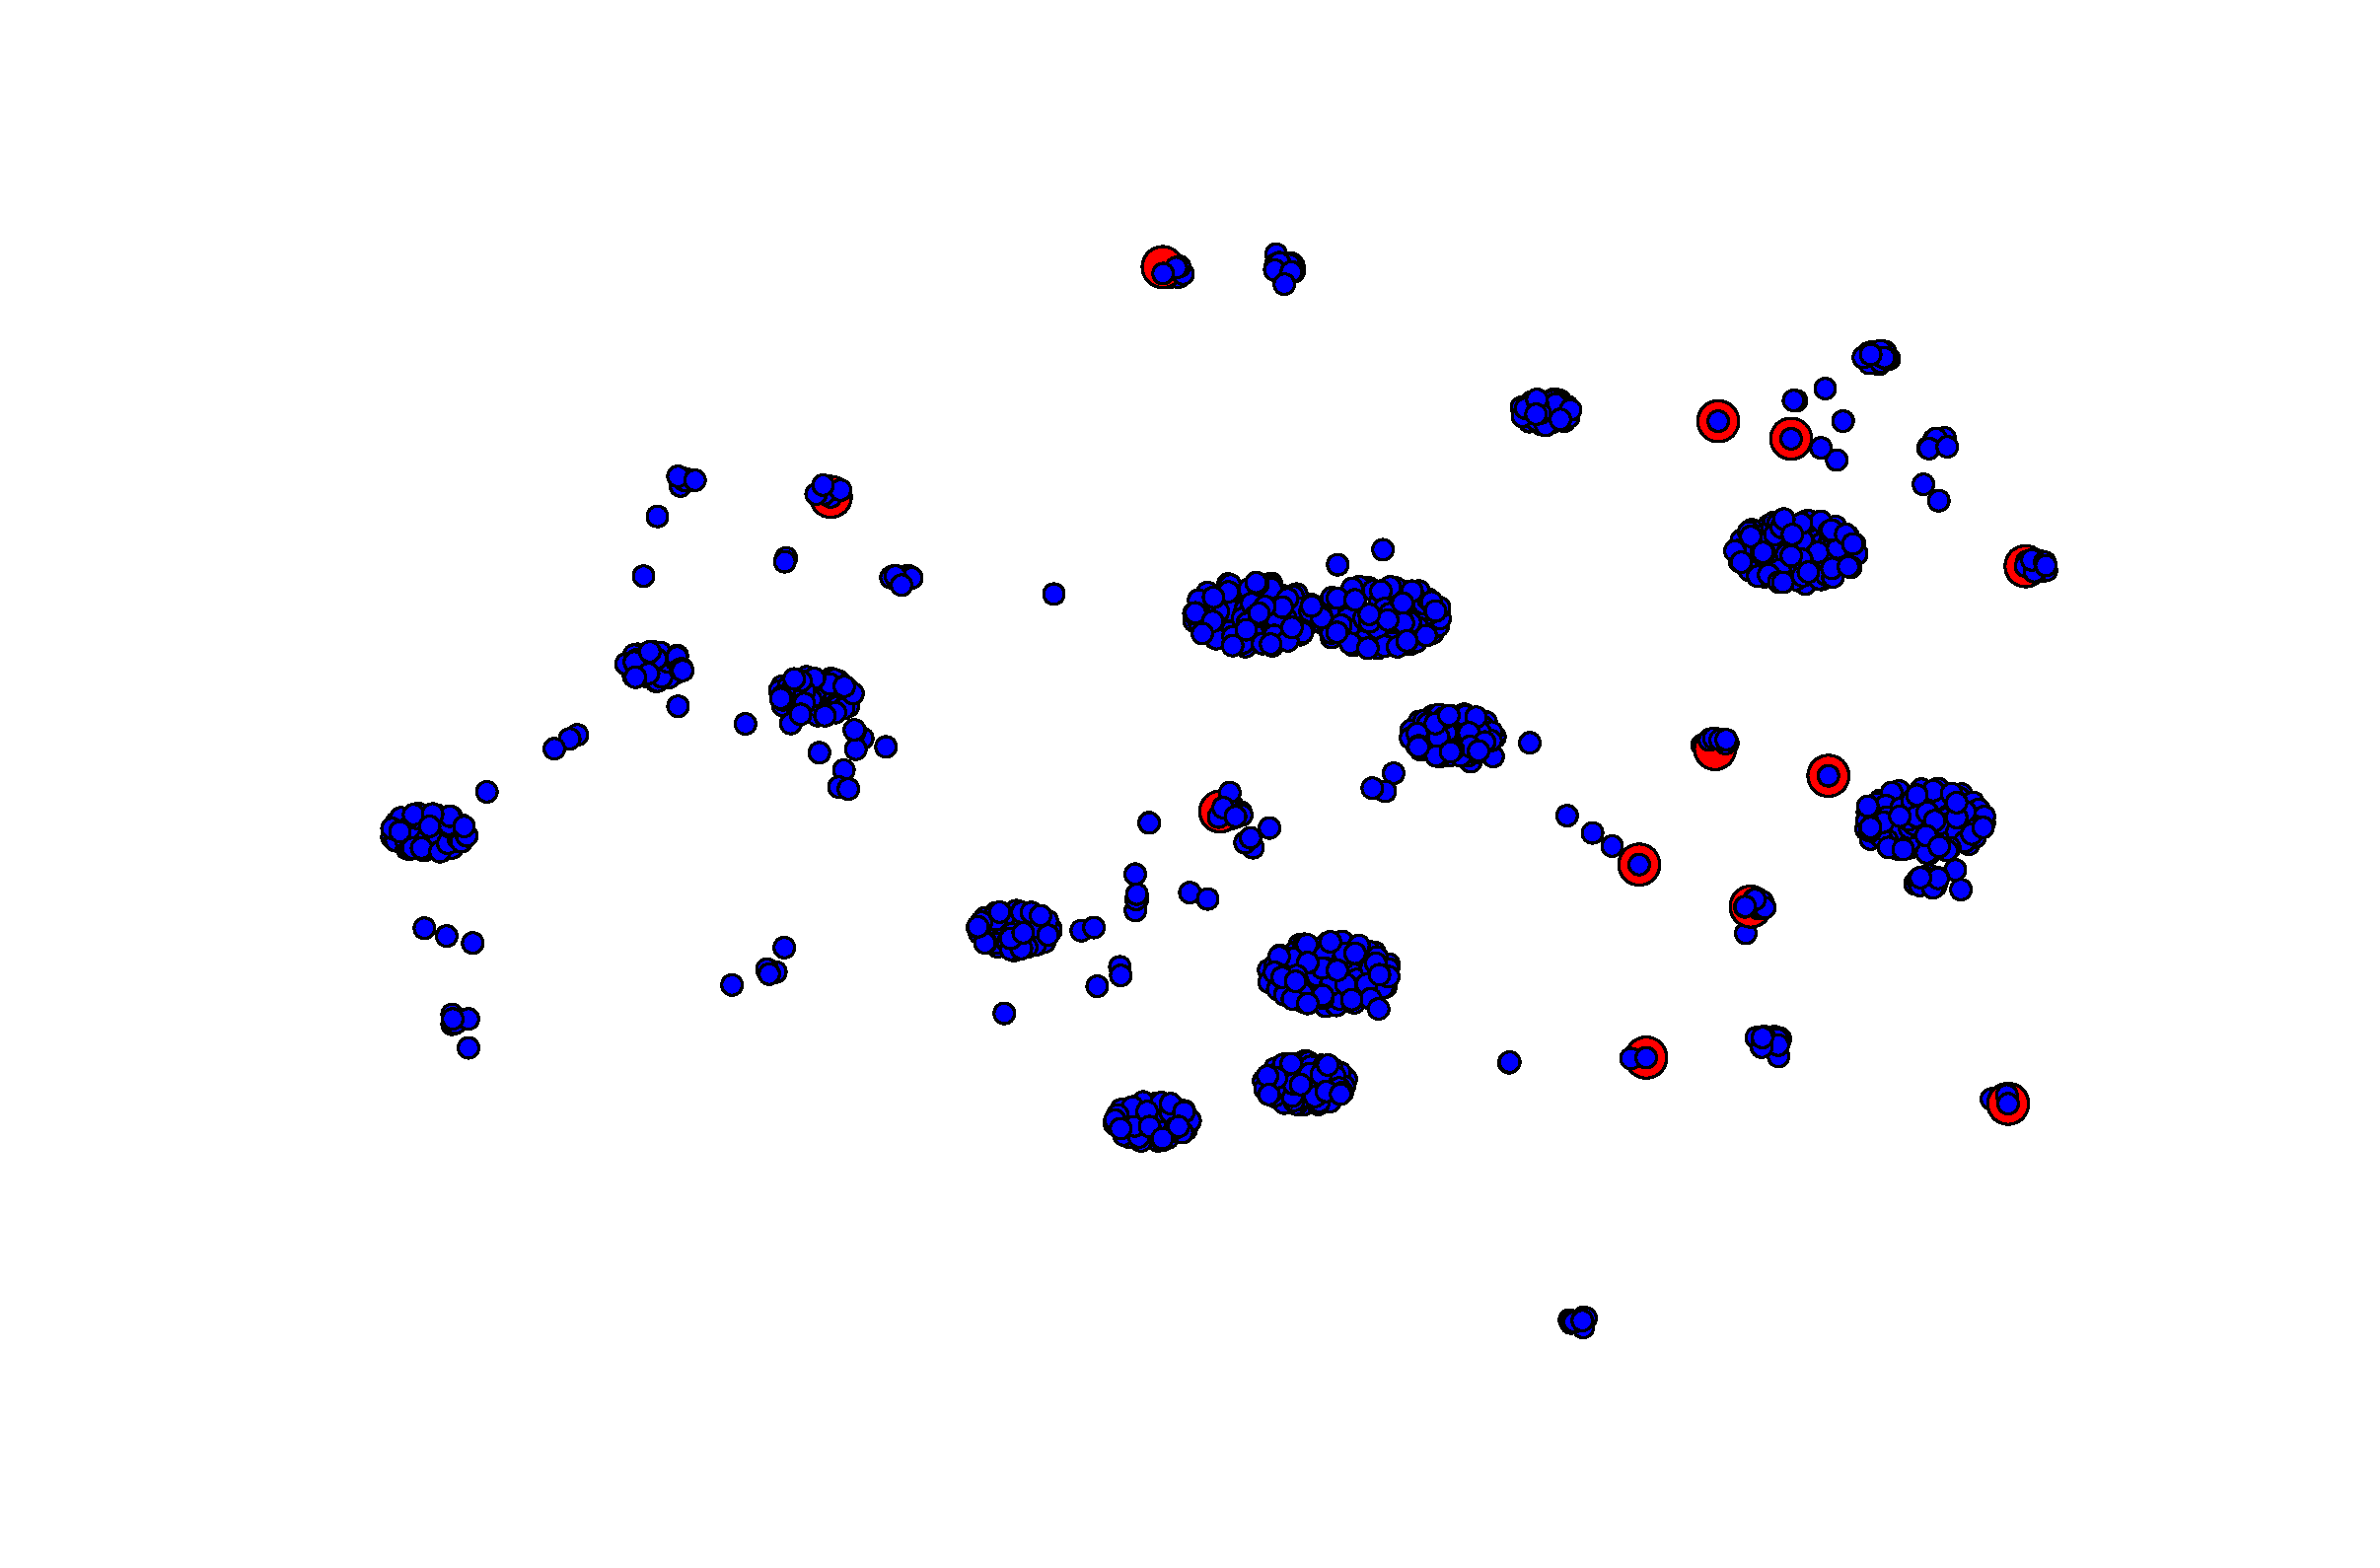
\includegraphics[width =1\textwidth]{tsne_1chord_transpositions.eps}
\caption{Representation of chords (blue dots), using T-Sne. A chord is transposed to all the possible pitches, which corresponds to the twelve red dots.}
\label{results1}
\end{figure}

We can see on figure \ref{results1}, that the blue dots tend to make clusters, showing that the network is able to organize the data. The transposition of the same chord were already contained in the dataset, as the red dots coincide with blue dots. Here, neither the PCA nor the T-SNE provided relevant layouts of the red dots. From a musical point of view, this can be understood as such : randomly transposing a chord doesn't create much harmony, this need to be done in a more subtle way. Also sometimes, only transposing is not enough, the third may need to go from major to minor for example. 

Considering this, we chose to highlight an other group of chord, hoping that this time we could visualize some interesting layout. Thus we chose the chords contained in Eiffel65 - I'm Blue, which undoubtedly make musical sense. Here, we were glad to see that the PCA visualization aligned the four different chords contained in the progression, meaning that our embedding space make sense (see figure \ref{fig:results2}).

\begin{figure}[H]
\centering
\includegraphics[width =1\textwidth]{T_Sne_Eiffel.png}
\caption{Representations of the chord progression of Eiffel65 - I'm Blue (red dots) in our embedding space : PCA on the left, T-Sne on the right.}
\label{fig:results2}
\end{figure}

The PCA algorithm spreads the dot but seems to give sense to musical progression ; whereas the T-Sne clusters the dots but doesn't put the chords of a progression on a simple geometric figure.

\section{To go further}

\subsection{Frame-level Accuracy}

As a reminder, the output of our networks is currently a midi vector of dimension $128 \times 1$ containing the prediction of the chord to come. But the data we want to predict is particularly sparse (3 or 4 bins out of 128 are non-zero). So there is a risk that the network predicts only zeros in order to minimize the MSE.

A way to avoid that is to use another cost function, for example the \textit{frame-wise accuracy}. It relies on the count of false positives, false negatives and true positives, ignoring the true negatives. The exact formula is given at : \href{http://citeseerx.ist.psu.edu/viewdoc/download?doi=10.1.1.205.9184&rep=rep1&type=pdf}{accuracy}.

We were able to implement this function, but it contains non-differentiable operations like thresholds, maxima ... so we were not able to back-propagate the gradient and train the network with it. The main obstacle is that the frame-level accuracy requires integer inputs, and forcing the network to output only integer necessary introduces non differentiable operations. But the measure remains available in our models as a performance indicator.

\subsection{Attention}
To improve the efficiency of our LSTM, it is possible to implement something called "attention". This allows our network to focus on the most relevant past notes/chords, as some of them may be a better indicator of the harmonic structure of the progression. This can be done combining two RNNs, with one of them learning to optimally read the output of the other one.

The application in image recognition is pretty obvious : if a dog is sitting on a chair, it's easier for the algorithm to first focus on the dog, and then on the chair, rather than identifying them both as the same time. There are indeed two networks needed to proceed this task : one to chose what area needs to be focused on, and an other to recognize what's inside the chosen area.

The effect of such an algorithm on our midi sequences is uncertain, but we can make some guesses : maybe it would select the most useful part of the score by recognizing the musical structure of the piece, as it recognizes the structure of a picture when applied to it. For example, when trying to predict a note from a refrain, it's more relevant to focus the attention on an other refrain  (see figure \ref{attention_adams}).

\begin{figure}[H]
\centering
\includegraphics[width =1\textwidth]{attention.png}
\caption{Clavinet midi file from \textit{The Adams Family} theme.
As a new musical phrase is starting, the best thing to do in order to predict the incoming note is to focus on the last time the same phrase was encountered.}
\label{attention_adams}
\end{figure}

\subsection{Usages for musical creativity}
We have seen that with embedding spaces we can predict from a set of chords a following chord. So it is easy to figure out that our model could help players improvising on live sets. The tricky issue would be the real-time question. So let’s put the idea of live set aside. And this leads us to a producing application: helping composers when working on a new creation. The composer can just input the beginning of a new song and the style of music he is composing, and the model will release a chord fitting with the composer’s expectations. Obviously, the application will just give a suggestion that the composer is free to consider in his work.

Given that the model takes care of the musical style, we can imagine that if we train it with rhythms from existing songs, it will be able to suggest typical rhythms from what it learned. This way, we are provided with a new typical rhythm that may be the base of a new song. With these two examples, we see that we can easily figure out plenty of composition applications.

\section{Conclusion}

This project was an interesting opportunity to raise many questions about harmony and musical structures organization. We explored many hypotheses, trying to rely as much as possible on actual music scores. This helped us make decisions about how to build and extend our own dataset. In the end, it's obviously not as wide as those used in big companies, but it already made it possible for us to train some neural networks. 

To improve our chance of getting satisfying results, we implemented both recurrent and convolutional neural networks. Though their validation rate can seem quite modest for the moment, it is actually very encouraging, considering how hard it is to predict a chord and how the dataset was crafted. Work would still be needed to make deep connections between the output of the networks and musical theory, as this project is more to be seen as a first approach to such a broad topic.

\bibliographystyle{alpha}
\bibliography{ml.bib}

\end{document}


